\section{Problem Definition}
In this work, we focus on sampling under the network crawling scenario.  For example, suppose that we want to obtain data from Twitter, and we have only 24 hours to collect the data. The goal is to get as many users as possible. The process starts by selecting one known user account. Then, we send a request through the API asking for the followers of this account. The server responses by returning a list of users back.  All the users are stored in the list, and our next query must be selected from this list.  At each step, the node we query must be one observed from a previous query.  The output is a set of unique users in the list.

\textit{Definition:} Suppose there is a true, underlying undirected network $G(V,E)$, where $V$ is set of nodes (users), $E$ is a set of edges (activities).  We assume that we have no information about $G$.  We are given a starting node$(n_{start})$ and a number of API requests $(budget)$. We are allowed to send a request to an API asking for neighbors of the specified node. The API returns all neighbors of the queried node. Our goal is to collect a sample graph $S(V',E')$, $V' \subseteq V$ and $E' \subseteq E$, where the number of nodes in $|V'|$ is maximized. 


\section{Proposed Method}
In this section, we introduce the novel sampling algorithm \textit{\ref{algo-name}}.  The current state-of-the-art algorithm, Maximum Observed Degree, in each step queries the node with the highest observed degree, with the assumption that this node has high unobserved degree as well.  \ref{algo-name} is based on the intuition that real networks exhibit community structure, and so if one queries the node with the highest observed degree, one may get `stuck' in a community.  \ref{algo-name} thus consists of two phases: \textit{Densification}, which queries nodes in the observed region to fill out that region, and \textit{Expansion}, which transitions the sampling algorithm to a new region of the graph.

For example, suppose the data collection process starts at a node in the bottom-left cluster in Figure \ref{fig:example}. As we can see, this network has several communities. The green area is already explored, and the sample obtained so far is from this region. The rest are the nodes have not been seen yet. The Densification phase aims to collect as many nodes that are densely connected. When the algorithm collects most of the nodes in that region, the algorithm switches from Densification to Expansion. The Expansion phase aims to escape from the current region. It picks an appropiate node that will lead to a new region. The algorithm switches between these two phases until it runs out of the budget. Pseudocode is shown in Algorithm \ref{exp-den} and a list of variables in Table \ref{tab:notation}.

\newcommand*{\captionsource}[2]{%
  \caption[{#1}]{%
    #1%
    \\\hspace{\linewidth}%
    (source: #2)%
  }%
}

\begin{figure}[h]
    \centering
    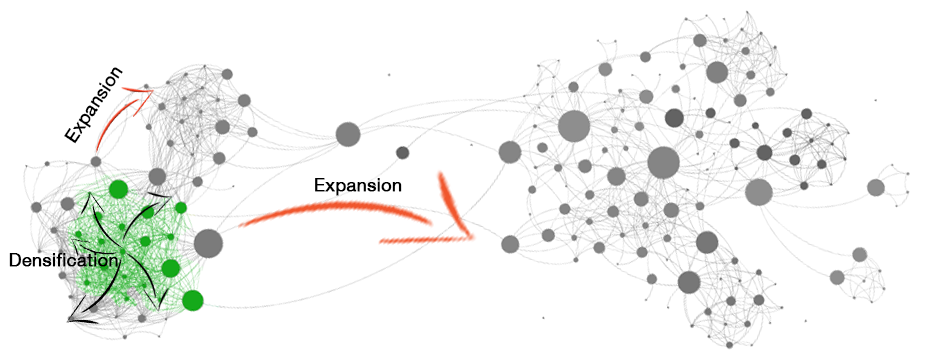
\includegraphics[width=0.5\textwidth]{concept}
    \caption{Concept of Expansion-Densification Algorithm}
    \label{fig:example}
\end{figure}

Algorithm \ref{exp-den} starts by collecting a small sample. The initial sample can be collected by any crawling technique. In our case, we adopt BFS crawling as shown in line 2.  BFS begins from any node $n_{start}$, queries the API for the node's neighbors, and adds all neighbors that have not been queried to an $\textit{unqueried}$ queue. The first node in the queue will be a next selected node. BFS is repeated for $budget_{bfs}$ times. All the nodes and edges found are kept as the initial sample. We define two types of nodes, $\textit{closed}$ and $\textit{open}$ node. A
$\textit{closed node}$ is a node that has already been queried. An $\textit{open node}$ is a node that has been observed, but not queried.

The main loop (line 3-7) of the algorithm switches between $Expansion$ and $Densification$, and it runs until it reaches a specified amount of budget. The input for $Expansion$ is the sample graph that obtained so far, and it returns a single node ($n_{exp}$), with the hope that $n_{exp}$ leads to a new region. $Densification$ acquires $n_{exp}$ as its input and tries to explore this new area of the network. It returns the sub-sample graph($S_{s}$). Finally, $S_{s}$ is merged with $S$.





\begin{algorithm}
\small
\caption{Exp-Den ({$budget, budget_{bfs}, n_{start}$})}\label{exp-den}
\begin{algorithmic}[1]
%\Function{Exp-den}{$budget, budget_{bfs}, n_{start}$}
\State $cost \gets 0$
\State $S \gets bfs(budget_{bfs}, n_{start})$ 
\While  {$cost \leq budget$}
	\State $n_{exp} \gets Expansion(S)$
	\State $S_{s} \gets Densification(n_{exp})$
	\State $S \gets $ Merge $S_{s}$ with $S$
\EndWhile
\end{algorithmic}
\end{algorithm}

\begin{center}
	\captionof{table}{Description of each variable} \label{tab:notation} 
    \begin{tabular}{  l | l }
    \hline
	 &  Description \\ \hline
	$N_{q}$ & a set of nodes returned from the API request\\
	$E_{q}$ & a set of edges returned from the API request\\
	$S$ & a sample graph $S(V',E')$ \\
	$S^{o}$ & a set of open nodes $n \in V'$\\
	$S^{c}$ & a set of closed nodes $n \in V'$\\
	$S_{s}$ & a sub-sample graph $S_{s}(V_{s},E_{s})$\\
	$S_{s}^{o}$ & a set of open nodes $n \in V_{s}$\\
	$S_{s}^{c}$ & a set of closed nodes $n \in V_{s}$\\
	$e_{ij}^{'}$ & $e_{ij} \in E_{s},(i \in S_{s}^{c} \wedge j \in S_{s}^{o})\vee(i \in S_{s}^{o} \wedge j \in S_{s}^{c}) $ \\
	$sc_{exp}^{t}$ & an expansion score at $t^{th}$ iteration \\
	$sc_{den}^{t}$ & a densification score at $t^{th}$ iteration \\
	$n_{exp}$ & a selected node from Expansion phase \\
	$w_{1}, w_{2}$ & weight \\	
	%$n_{c_{i}}$ & a set of nodes in $i^{th}$ community \\
	%$d_{c_{i}}$ & a diameter of $i^{th}$ community\\
	$|\cdot|$ & a cardinality of a set \\ \hline
    \end{tabular}
    
\end{center}


\begin{algorithm}
\caption{Densification ({$n_{cur}$})}\label{mod}
\begin{algorithmic}[1]
%\Function{MOD}{$n_{cur}$}
\State $S_{s} \gets empty$, $sc^{0}_{den} \gets 1$, $sc^{0}_{exp} \gets 0$
%\State $sc^{0}_{den} \gets 1$, $sc^{0}_{exp} \gets 0$
%\State $sc^{0}_{exp} \gets 0$\Comment{Set Expansion score to 0 }
\While {$sc^{t}_{exp} < sc^{t}_{den}$ or $cost < budget$}
	\State $N_{q}, E_{q} \gets $Make a query on $n_{cur}$
	
	\State $sc^{t}_{den} \gets w_{1}\times \frac{ \vert n \in N_{q} \backslash (S^{o} \cup S_{s}^{o} ) \vert }{\vert S_{s}^{c} \vert} + w_{2} \times sc^{t-1}_{den}$
	
%e(i,j) \in S_{s}^{e},(i \in S_{s}^{c} \wedge j \in S_{s}^{o})\vee(i \in S_{s}^{o} \wedge j \in S_{s}^{c}) 	
	
	\State $sc^{t}_{exp} \gets w_{1} \times  \frac{\vert e^{'}_{ij} \vert }{\vert S_{s}^{o} \vert}  + w_{2} \times sc^{t-1}_{exp}$
	\State $S_{s} \gets $ Add $N_{q}, E_{q}$ to sub sample
	\State $n_{cur} \gets $node with the highest degree in $S_{s}$
	\State $cost \gets cost + 1 $
\EndWhile

\Return $S_{s}$
%\EndFunction
\end{algorithmic}
\end{algorithm}

%\begin{algorithm}
%\caption{Expansion ({$S$})}\label{oracle}
%\begin{algorithmic}[1]
%	\For {$c_i $  in $C$}
%		\State $score_{i} \gets \frac{\vert n_{c_i} \vert}{|V|} \times  \frac{1}{d_{c_i}}$  \Comment{ score = gain x spread}
%	\EndFor
%	\State $ C_{target} = argmax(score_{i})$
%	
%	\For {$n $  in $S^{o}$}
%		\State $d_{n} \gets $ shortest path length from $n$ to $C_{target}$
%	\EndFor	
%	\State $ n_{best} = argmin(d_{n})$
%
%\Return $n_{best}$
%\end{algorithmic}
%\end{algorithm}



\textbf{Densification: }
To expand a sample within a region, we adopt Maximum Observed Degree (MOD)\cite{avrachenkov2014pay}, as it outperforms other algorithms in the same class. Pseudocode is shown in Algorithm \ref{mod}. In each iteration, the node with maximum degree is selected from $S_{s}^{o}$ and the algorithm requests its neighbors through the API. Nodes ($N_{q}$) and edges($E_{q}$) are returned and added to sub-sample ($S_{s}$). 

\textbf{Expansion: } In the Expansion step, the algorithm tries to escape from the current region of the network. The algorithm selects a node that will lead to another dense area. In the spirit of explore-exploit algorithms, one naive appoarch is to pick a node uniformly at random from $S^{o}$.  We refer this Expansion strategy as ``$random$" (in our future work, we examine other strategies for Expansion). 

\textbf{Switching Phases:}
Two scores are calculated in each iteration of Densification. Intuitively, in each step, the number of closed nodes increases while a number of new nodes added decreases over time (diminishing marginal returns). The algorithm will find many nodes in the same community at the beginning and this amount drastically drops when most of them are found. $sc^{t}_{den}$ measures how many new nodes are added to the sample after a request, divided by the number of closed nodes.  $sc^{t}_{exp}$ is the fraction of the number of edges ($e_{ij}^{'}$) connecting a closed node to an open node, divided by the number of open nodes in sub-sample.  If the number of edges $(e'_{ij})$ increases, the number of open nodes also increases. If not, it means the algorithm already found most of the nodes.  These scores give us an approximation of number of nodes left unexplored. Densification switches to Expansion when $sc^{t}_{exp}$ is higher than $sc^t_{den}$. Thus, the algorithm can appropiately switch between phases. 

%\textbf{Expansion: } In the Expansion step, we want to escape from the current part of the network. The algorithm selects a node in order to explore on another dense area. One naive appoarch is to pick one node uniformly at random from $S^{o}$, we refer this Expansion strategy as "$random$". Moreover, we introduce another appoarch, we refer as "$\textit{Oracle}"$. We assume that Oracle has the information of the entire graph. The pseudocode is shown in Algorithm \ref{oracle}. Firstly, Oracle selected a target community($C_{t}$) by considering the score (line 1-3). A community with the highest score is selected. The score is a multiplication of $gain$ and $spread$. $Gain$ measures a number of nodes left unexplored. $Spread$ measures how fast we can reach all the nodes in the community. We define spread is inversely proportional to the diameter of community($d_{c_{i}}$). After target community is selected, Oracle calculates the shortest path length from every open nodes($S^{o}$) to the target community. A node with the smallest distance is selected. Note that, we can improve the performance here by calculating clustering coefficient of all nodes in $S^{o}$ and ignore all node that the clustering coeffocient is equal to one. It is likely that these nodes are in the same community since the neighbors are tightly connected.
